\chapter{Domain and Element Configuration} \label{chap:domainconfig}

A domain and all its topological elements as well as the underlying geometric space are specified in a common configuration class.
The setup of such a configuration class is explained in detail in Section \ref{sec:config-class}.

Even though mathematically all $n$-cells of a domain are well defined and available on paper, it may not make sense to store explicit representations of these elements in memory.
For example, a particular algorithm may not required the storage of edges and/or facets of a domain, thus keeping them in memory can be a considerable waste of resources.
Section \ref{sec:customizing-storage} explains how the underlying storage scheme of {\ViennaGrid} can be adjusted to the library user's requirements and to be as memory-efficient as possible.


\section{The Configuration Class} \label{sec:config-class}
A valid configuration class for {\ViennaGrid} is any class that provides the following three public member types:
\begin{center}
\begin{tabular}{|l|p{8cm}|}
\hline
 \lstinline|numeric_type|   & The underlying scalar type of the geometric space. \\
\hline
 \lstinline|coordinate_system_tag| & A tag specifying the underlying coordinate system.\\
\hline
 \lstinline|cell_tag|       & A tag that identifies the cell type inside the domain.\\
\hline
\end{tabular}
\end{center}

More details on the types are given in the following:
\begin{itemize}
 \item \lstinline|numeric_type|: This refers to the type of the coordinates of a point in the geometric space. In most cases, one may want to use \lstinline|double|. However, it may also be the case that the user prefers to use integer coordinates, or high-precision floating point libraries such as ARPREC \cite{arprec}.

 \item \lstinline|coordinate_system_tag|: Any of the following predefined classes from namespace \lstinline|viennagrid| can be defined as \lstinline|coordinate_system_tag| to select the coordinate system of the underlying geometric space:
   \begin{center}
   \begin{tabular}{|l|l|}
    \hline
    \lstinline|cartesian_cs<dim>|   &  Cartesian coordinate system of dimension \lstinline|dim| \\
    \hline
    \lstinline|polar_cs|       &  Polar coordinate system in two dimensions \\
    \hline
    \lstinline|spherical_cs|   &  Spherical coordinates in three dimensions \\
    \hline 
    \lstinline|cylindrical_cs| &  Cylindrical coordinates in three dimensions \\
    \hline
   \end{tabular}
   \end{center}

 \item \lstinline|cell_tag|: A tag that specifies the type of the elements with maximum topological dimension in the domain. The following two families of topological elements are provided with {\ViennaGrid} in namespace \lstinline|viennagrid|:
   \begin{center}
   \begin{tabular}{|l|l|}
    \hline
    \lstinline|simplex<n>|     &  Refers to an $n$-simplex \\
    \hline
    \lstinline|hypercube<n>|   &  Refers to an $n$-hypercube \\
    \hline
   \end{tabular}
   \end{center}
 It should be noted that \lstinline|simplex<1>| and \lstinline|hypercube<1>| both refer to a line segment. Typical examples from these families for common values of $n$ are as follows:
   \begin{center}
   \begin{tabular}{|l|l|}
    \hline
    \lstinline|simplex<2>|     &  Triangle \\
    \hline
    \lstinline|simplex<3>|     &  Tetrahedron \\
    \hline
    \lstinline|hypercube<2>|   &  Quadrilateral \\
    \hline
    \lstinline|hypercube<3>|   &  Hexahedron \\
    \hline
   \end{tabular}
   \end{center}
 The reference orientations of these cells can be found in the Appendix.
\end{itemize}

All geometric and topological types are then derived from the configuration class. To this end, {\ViennaGrid} provides
a number of metafunctions that reside in namespace \lstinline|viennagrid::result_of|. The naming follows the conventions in the Boost libraries \cite{boost}.
For a configuration class \lstinline|Config|, the respective types are obtained as follows:
\begin{lstlisting}
 using namespace viennagrid;

 typedef result_of::domain<Config>::type     DomainType;
 typedef result_of::segment<Config>::type    SegmentType;
 typedef result_of::ncell<Config, 0>::type   VertexType;
 typedef result_of::ncell<Config, 1>::type   EdgeType;
\end{lstlisting}
In particular, the type of any $n$-cell is obtained as
\begin{lstlisting}
 typedef result_of::ncell<Config, n>::type   ElementType;
\end{lstlisting}
where $n$ has to be replaced with the respective value. This allows to formulate algorithms such as domain boundary detection in a very general manner and can be used for recursively iterating through the $n$-cells of different dimension. In order to obtain the types of cells and facets, one should use the topological dimension from the cell tag:
\begin{lstlisting}
 typedef Config::cell_tag                                CellTag;
 typedef result_of::ncell<Config, CellTag::dim-1>::type  FacetType;
 typedef result_of::ncell<Config, CellTag::dim>::type    CellType;
\end{lstlisting}


\TIP{Please note that in template classes and template functions one needs to add an extra \lstinline|typename| after each \lstinline|typedef| keyword in the code snippets above.}



\section{Customizing Storage of $n$-Cells} \label{sec:customizing-storage}
One of the outstanding features of {\ViennaGrid} over other libraries related to grid handling is the possibility to customize the internal storage of elements. By default, all $n$-cells of a domain are stored explicitly inside the domain. In addition, each $n$-cell stores links to its boundary $k$-cells, with $k<n$. While this overhead is not a concern for topologically one-dimensional meshes and moderate for topologically two-dimensional meshes, it can be a considerable issue for dimensions three and above. 

As an example, linear finite elements need information about the cells and the vertices inside the domain, while edges and facets may not be needed depending on the boundary conditions imposed.

\begin{table}[tb]
 \centering
 \begin{tabular}{|l|r|r|r|}
  \hline
         & Amount      & Bytes/Object         & Total Memory \\
  \hline
  Vertices & 4913 & 24 & 115 KB \\
  \hline
  Edges   & 31024 & 16 & 485 KB \\
  \hline
  Facets  & 50688 & 48 & 2376 KB \\
  \hline
  Cells   & 24576 & 112 & 2688 KB \\
  \hline
  \textbf{Total}  &       &     &  \textbf{5664 KB} \\
  \hline
 \end{tabular}
 \caption{Minimum memory consumption for a tetrahedral mesh of the unit cube where all $n$-cells are stored explicitly and boundary information on each $n$-cell is stored. Vertices use \lstinline|double|-precision coordinates and elements are linked with pointers sized eight bytes each.}
 \label{tab:full-domain-memory}
\end{table}

\begin{table}[tb]
 \centering
 \begin{tabular}{|l|r|r|r|}
  \hline
         & Amount      & Bytes/Object         & Total Memory \\
  \hline
  Vertices & 4913 & 24 & 115 KB \\
  \hline
  Edges   & 0 & - & 0 KB \\
  \hline
  Facets  & 0 & - & 0 KB \\
  \hline
  Cells   & 24576 & 32 & 768 KB \\
  \hline
  \textbf{Total}  &       &     &  \textbf{883 KB} \\
  \hline
 \end{tabular}
 \caption{Minimum memory consumption for a tetrahedral mesh of the unit cube where only $0$-cells and $3$-cells are stored explicitly. $3$-cells have knowledge of their $0$-cells only. Vertices use \lstinline|double|-precision coordinates and elements are linked with pointers sized eight bytes each.}
 \label{tab:slim-domain-memory}
\end{table}

As shown in Tab.~\ref{tab:full-domain-memory} and Tab.~\ref{tab:slim-domain-memory}, storing facets and edges explicitly increases the total memory consumption by a factor of more then six. In cases where additional maps for the mapping from local to global $n$-cell orientations are stored together with the topological boundary information, the difference in memory consumption is above one order of magnitude.

\NOTE{Note that in {\ViennaGrid} a cell always stores pointers to its vertices. Similarly, the domain always stores the cells and vertices.}

{\ViennaGrid} can be customized to switch seamlessly between the different storage models, as will be shown in the following subsections.

\subsection{Boundary $n$-Cells} \label{subsec:boundary-ncells-storage}

This can be achieved in two ways:
\begin{itemize}
 \item \textbf{Method 1}: Use the provided macros. The storage of elements can be customized either for a particular configuration class, or globally for all domain configuration classes. To disable the storage of edges (i.e.~$1$-cells) inside a tetrahedron for a domain with configuration class \lstinline|MyConfig|, the line
  \begin{lstlisting}
VIENNAGRID_DISABLE_BOUNDARY_NCELL(MyConfig,
                                  viennagrid::tetrahedron_tag, 1)
  \end{lstlisting}
right after the {\ViennaGrid}-includes in the source file containing \lstinline|main()| is sufficient. Make sure that the macro is placed in the global namespace. The first argument is the configuration class, the second class is the tag for the respective $n$-cell for which the boundary element should be disabled, and the third parameter is the topological dimension for which the handling should be disabled.
 If no edges should be stored for a tetrahedron irrespective of the configuration class, the macro
  \begin{lstlisting}
VIENNAGRID_GLOBAL_DISABLE_BOUNDARY_NCELL(viennagrid::tetrahedron_tag,
                                         1)
  \end{lstlisting}
 should be used. If one wishes to selectively enable the handling of boundary cells within a globally disabled environment, one can use e.g.
  \begin{lstlisting}
VIENNAGRID_ENABLE_BOUNDARY_NCELL(MyConfig,
                                 viennagrid::tetrahedron_tag, 1)
  \end{lstlisting}
 to enable the storage of edges inside a tetrahedron.

 \item \textbf{Method 2}: The macros above are shortcuts for class specializations. The first two macros expand to the following code:
\begin{lstlisting}
namespace viennagrid { namespace result_of {
    template <>
    struct subelement_handling<MyConfig,
                               viennagrid::tetrahedron_tag, 1>{
      typedef no_handling_tag    type;
    };

    template <typename ConfigType>
    struct subelement_handling<ConfigType,
                               viennagrid::tetrahedron_tag, 1>{
      typedef no_handling_tag    type;
    };
} }
\end{lstlisting}
The third macro explained for method 1 results in the same code as the first macro, with the exception that \lstinline|no_handling_tag| is replaced with \lstinline|full_handling_tag|.

Finally, we wish to point at a potential pitfall when disabling $n$-cells that are neither $0$-cells, $N-1$-cells nor $N$-cells: As example, we consider the case of disabling edges for a tetrahedron. Using the line
  \begin{lstlisting}
VIENNAGRID_DISABLE_BOUNDARY_NCELL(MyConfig,
                                  viennagrid::tetrahedron_tag, 1)
  \end{lstlisting}
only disables the edges for the tetrahedron, but still edges are pushed and stored inside the domain because the triangular facets of the tetrahedron store pointers to their edges. Thus, to completely disable the storage of any edges, one also has to disable the storage of edges for triangles. As a check, one should verify that the number of edges stored inside a domain \lstinline|my_domain| and obtained by 
 \begin{lstlisting}
  viennagrid::ncells<1>(my_domain).size()
 \end{lstlisting}
is zero.

\TIP{Have a look at \texttt{examples/tutorial/slim\_domain.cpp} and selectively enable or disable the storage of elements to see the impact on total memory consumption. Note that the bytes per object may differ from Tab.~\ref{tab:full-domain-memory} and Tab.~\ref{tab:slim-domain-memory} depending on the use of local-to-global-orienters and the eventual use of integral IDs.}

\subsection{Local Orientations}
\begin{figure}[tb]
\centering
 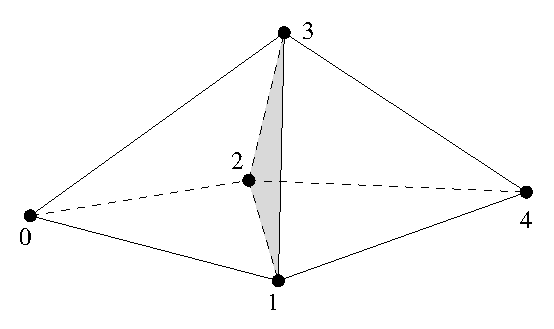
\includegraphics[width=0.65\textwidth]{figures/interface-tets.eps}
 \caption{Boundary $n$-cells have different orientations with respect to different cells.}
 \label{fig:orientation-boundary-ncells}
\end{figure}

In cases where $n$-cells store boundary $k$-cells, $k<n$, it may be required to know the orientation of the globally (i.e.~in the domain) stored $k$-cell with respect to the local reference orientation of the $n$-cell. The common facet of the two tetrahedra in Fig.~\ref{fig:orientation-boundary-ncells} may be stored globally using the sequence of vertex indices $[1, 2, 3]$. Inside the tetrahedron $[0, 1, 2, 3]$ the facet again possesses the orientation $[1, 2, 3]$, thus matching the global orientation. However, within the tetrahedron $[4, 2, 1, 3]$ the facet has the local orientation $[2, 1, 3]$ (refer to the Appendix for an overview of reference orientations). For applications such as high-order finite elements, such a local orientation with respect to the cell is required.


By default, {\ViennaGrid} stores the local orientation of each boundary $k$-cell inside the hosting $n$-cell. In order to disable the storage of these local orientations for scenarios where the local orientation is not needed, there are again two methods provided:
\begin{itemize}
 \item \textbf{Method 1}: Using the macros provided. To disable the storage of local orientations of edges (i.e.~$1$-cells) inside a tetrahedron for a domain with configuration class \lstinline|MyConfig|, the line
\begin{lstlisting}
VIENNAGRID_DISABLE_BOUNDARY_NCELL_ORIENTATION(MyConfig,
                           viennagrid::tetrahedron_tag, 1) 
\end{lstlisting}
is sufficient. The second argument denotes the hosting $n$-cell tag, while the third argument denotes the topological dimension $k$ of the boundary $k$-cells.

Similar as in the previous section, one can disable the storage of local orientations globally for all configuration classes by
\begin{lstlisting}
VIENNAGRID_GLOBAL_DISABLE_BOUNDARY_NCELL_ORIENTATION(
                              viennagrid::tetrahedron_tag, 1) 
\end{lstlisting}
To selectively enable the storage of local orientation in a globally disabled setting, the macro \lstinline|VIENNAGRID_ENABLE_BOUNDARY_NCELL_ORIENTATION| can be used in the same way as \lstinline|VIENNAGRID_DISABLE_BOUNDARY_NCELL_ORIENTATION|.
Again, it is recommended to define the macros in the source file containing \lstinline|main()| after the inclusion of the {\ViennaGrid} header files.

 \item \textbf{Method 2}: Instead of using the macros, one can instead manually adjust the meta-function \lstinline|subelement_orientation|. The first macro of method 1 expands to
 \begin{lstlisting}
namespace viennagrid { namespace result_of {
  template <>
  struct subelement_orientation<MyConfig,
                                viennagrid::tetrahedron_tag, 1>
  {
    typedef no_handling_tag    type;
  };
}  }
 \end{lstlisting}
Using the type \lstinline|full_handling_tag| instead of \lstinline|no_handling_tag| enables the storage of local orientations.
\end{itemize}

\TIP{If the storage of boundary $k$-cells is disabled (cf.~Sec.~\ref{subsec:boundary-ncells-storage}), there are automatically no local orientations for boundary $k$-cells stored. The local orientations do not need to be disabled explicitly in this case.}

\subsection{$n$-Cell IDs}
It is often convenient to have enumerated $n$-cells within a domain such that every $n$-cell is aware of its index inside the random access container it resides in. This allows for some algorithms to use fast random-accesses with $\LandauO(1)$ costs rather than searching trees with $\LandauO(\log N)$ costs or linked lists with $\LandauO(N)$ costs, where $N$ here denotes the number of $n$-cells inside the domain. Conversely, if $\LandauO(\log N)$ access times are acceptable, then the memory for storing the container index (which we refer to in the following as \emph{$n$-cell ID}) is wasted. To accomodate for these two scenarios, {\ViennaGrid} allows to selectively enable or disable the storage of $n$-cell IDs. By default, $n$-cell IDs are stored, since they have negligible impact on the total memory consumption as soon as other boundary $k$-cells are stored for an $n$-cell.

As for the storage of boundary $k$-cells and local orientations, there are two possibilities for customizing the storage of IDs:
\begin{itemize}
 \item \textbf{Method 1}: Using the provided macros. To disable the storage of IDs for tetrahedrons inside a domain with configuration \lstinline|MyConfig|, the line
 \begin{lstlisting}
VIENNAGRID_DISABLE_NCELL_ID(viennagrid::config::tetrahedral_3d,
                            viennagrid::tetrahedron_tag)
 \end{lstlisting}
 is sufficient. The second argument denotes the element tag for which the storage of IDs should be disabled.

 To globally disable the storage of IDs for tetrahedrons, use
 \begin{lstlisting}
VIENNAGRID_GLOBAL_DISABLE_NCELL_ID(viennagrid::tetrahedron_tag)
 \end{lstlisting}
 To selectively enable the storage of IDs for certain configuration classes in a globally disabled setting, one can use
 \begin{lstlisting}
VIENNAGRID_ENABLE_NCELL_ID(viennagrid::config::tetrahedral_3d,
                           viennagrid::tetrahedron_tag)
 \end{lstlisting}

 \item \textbf{Method 2}:
The macros from the first method expand to
\begin{lstlisting}
 template <>
 struct element_id_handler<MyConfig, viennagrid::tetrahedron_tag>
 {
   typedef pointer_id    type;
 };
\end{lstlisting}
for the configuration class \lstinline|MyConfig|, and to
\begin{lstlisting}
    template <typename ConfigType>
    struct element_id_handler<ConfigType, viennagrid::tetrahedron_tag>
    {
      typedef pointer_id    type;
    };
\end{lstlisting}
for globally disabling the storage of IDs. To selectively enable IDs, \lstinline|integral_id| should be used instead of \lstinline|pointer_id|.


\end{itemize}



\TIP{Have a look at \texttt{examples/tutorial/slim\_domain.cpp} and selectively enable or disable the storage of elements, local orientations and IDs to see the impact on total memory consumption. Note that the bytes per object may differ from Tab.~\ref{tab:full-domain-memory} and Tab.~\ref{tab:slim-domain-memory} depending on the use of local orientations and integral IDs.}

\NOTE{Disabling $n$-cell IDs eliminates the possibility to store and access data for the respective $n$-cells with $\LandauO(1)$ costs, see Chapter [MISSING].}

\end{itemize}

